\chapter{Ejercicio Práctico N.º 2: Comunicación y Sincronización}
\label{sec.ej2:comunicacion}

\section{Descripción General}

El segundo ejercicio plantea la resolución del problema de productor-consumidor en un entorno con restricciones
temporales, integrando la adquisición de hardware mediante interrupciones con los mecanismos de sincronización
y pasaje de datos provistos por FreeRTOS.

El sistema debe adquirir de forma periódica una señal analógica conectada al canal 0 del convertidor analógico-digital
(pin PA0), transferir de manera segura la lectura hacia una tarea consumidora encargada de formatear y emitir el valor
digitalizado por el puerto serie USART1 cada $\SI{2000}{\milli\second}$, y mantener en paralelo la tarea de señalización
luminosa con el LED integrado en el pin PC13.

\section{Estructura de Tareas, Interrupciones y Prioridades}

La arquitectura del sistema divide las responsabilidades entre tres tareas independientes y una rutina de servicio
de interrupción (ISR) de hardware. En la tabla \ref{tab.ej2:tareas} se detallan sus atributos de ejecución.

\begin{table}[!ht]
\centering
\small
\caption{Atributos de tareas e interrupciones en el Ejercicio 2.}
\label{tab.ej2:tareas}
\begin{tabular}{llccl}
\toprule
Elemento & Tipo & Prioridad & Período & Función / Rol \\
\midrule
\texttt{vBlink} & Tarea & 3 & $\SI{100}{\milli\second}$ & Señalización en pin PC13 \\
\texttt{vReadADC} & Tarea & 2 & $\SI{100}{\milli\second}$ & Productor: disparo de ADC1 \\
\texttt{vSendTelemetry} & Tarea & 1 & $\SI{2000}{\milli\second}$ & Consumidor: cola y Tx USART1 \\
\texttt{ADC1\_2\_IRQHandler} & ISR & NVIC & Asíncrono & Lectura de ADC1 y despacho IPC \\
\bottomrule
\end{tabular}
\end{table}

El esquema de prioridades asignado responde a las siguientes consideraciones:

\begin{enumerate}
  \item \textbf{Prioridad 3 (\texttt{vBlink})}: Mantiene el nivel de prioridad más elevado para asegurar que la
  señalización luminosa del sistema no experimente variaciones de fase frente a las ráfagas de cómputo del convertidor
  o de la transmisión serie.
  \item \textbf{Prioridad 2 (\texttt{vReadADC}, Tarea Productora)}: Se programa con prioridad superior a la tarea de
  telemetría. Cada $\SI{100}{\milli\second}$ inicia la secuencia de muestreo en el periférico analógico escribiendo el bit
  de inicio por software (\texttt{ADC\_CR2\_SWSTART}). Al poseer prioridad 2, tiene precedencia sobre la tarea de
  telemetría si ambas estuvieran listas para ejecutarse simultáneamente.
  \item \textbf{Prioridad 1 (\texttt{vSendTelemetry}, Tarea Consumidora)}: Funciona con la prioridad más baja de las
  tareas de aplicación. Su activación ocurre cada $\SI{2}{\second}$ para retirar el dato más reciente de la cola y
  enviarlo por el canal serie, demandando mayor tiempo de CPU debido a la espera de los banderines de transmisión en
  el registro de estado de la USART.
  \item \textbf{Nivel de Interrupción (\texttt{ADC1\_2\_IRQHandler})}: Las interrupciones de periféricos operan por
  encima del nivel de tareas del sistema operativo, siendo administradas directamente por el controlador NVIC del
  núcleo Cortex-M3. Al completarse la conversión analógica, la ISR atiende de inmediato el evento, transfiriendo la
  información a las estructuras del sistema operativo sin demoras.
\end{enumerate}

En la figura \ref{fig.ej2:arquitectura} se representa el diagrama de bloques del sistema, detallando el flujo de
datos y las primitivas de sincronización empleadas.

\begin{figure}[!ht]
\centering
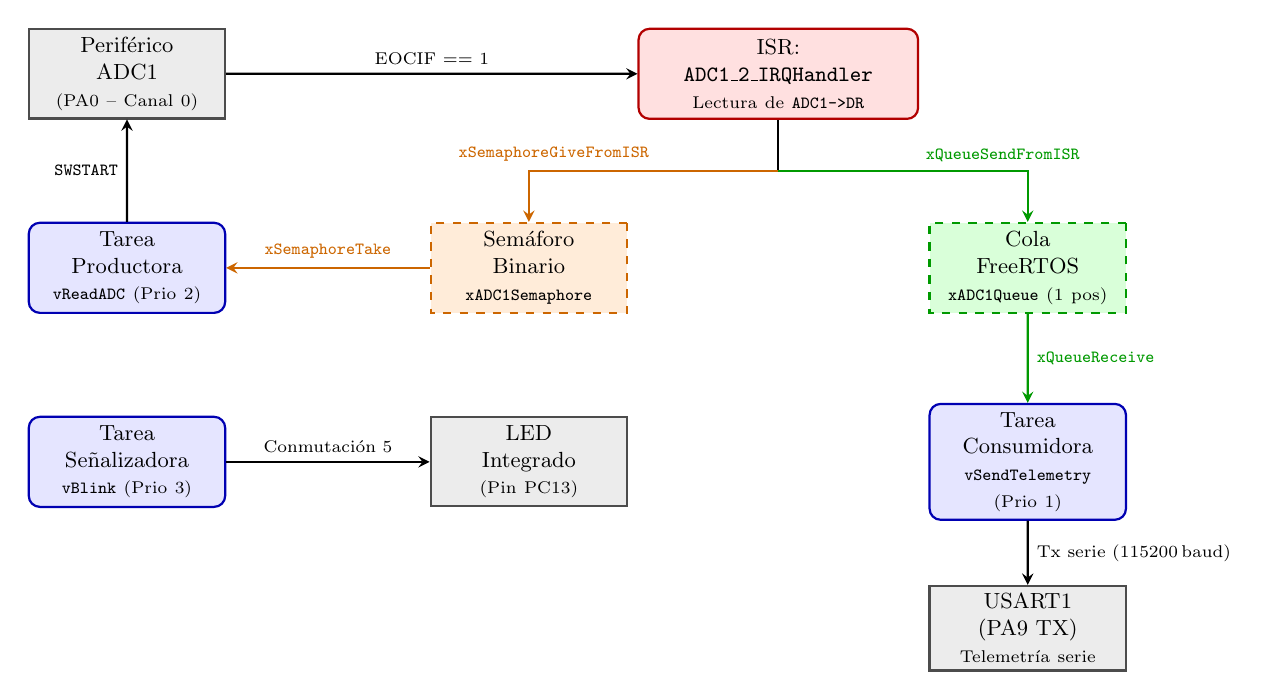
\begin{tikzpicture}[
    scale=0.88, transform shape,
    >=stealth,
    font=\small,
    block/.style={rectangle, draw=blue!70!black, thick, fill=blue!10, align=center, rounded corners=4pt, minimum height=1.3cm, text width=2.6cm},
    hw/.style={rectangle, draw=black!70, thick, fill=gray!15, align=center, minimum height=1.2cm, text width=2.6cm},
    isr/.style={rectangle, draw=red!70!black, thick, fill=red!12, align=center, rounded corners=4pt, minimum height=1.3cm, text width=3.8cm},
    queue/.style={rectangle, draw=green!60!black, thick, fill=green!15, dashed, align=center, minimum height=1.3cm, text width=2.6cm},
    sem/.style={rectangle, draw=orange!80!black, thick, fill=orange!15, dashed, align=center, minimum height=1.3cm, text width=2.6cm}
  ]

  % Fila 1: Periférico ADC e ISR (y = 4.2)
  \node[hw] (adc) at (0, 4.2) {Periférico\\ADC1\\{\scriptsize (PA0 -- Canal 0)}};
  \node[isr] (isr) at (9.4, 4.2) {ISR:\\\texttt{ADC1\_2\_IRQHandler}\\{\scriptsize Lectura de \texttt{ADC1->DR}}};

  % Fila 2: Tarea Productora y primitivas IPC (y = 1.4)
  \node[block] (task_prod) at (0, 1.4) {Tarea\\Productora\\{\scriptsize \texttt{vReadADC} (Prio 2)}};
  \node[sem] (sem) at (5.8, 1.4) {Semáforo\\Binario\\{\scriptsize \texttt{xADC1Semaphore}}};
  \node[queue] (queue) at (13.0, 1.4) {Cola\\FreeRTOS\\{\scriptsize \texttt{xADC1Queue} ($1$ pos)}};

  % Fila 3: Tarea Señalizadora, LED y Tarea Consumidora (y = -1.4)
  \node[block] (task_blink) at (0, -1.4) {Tarea\\Señalizadora\\{\scriptsize \texttt{vBlink} (Prio 3)}};
  \node[hw] (led) at (5.8, -1.4) {LED\\Integrado\\{\scriptsize (Pin PC13)}};
  \node[block] (task_cons) at (13.0, -1.4) {Tarea\\Consumidora\\{\scriptsize \texttt{vSendTelemetry} (Prio 1)}};

  % Fila 4: Periférico UART (y = -3.8)
  \node[hw] (uart) at (13.0, -3.8) {USART1\\(PA9 TX)\\{\scriptsize Telemetría serie}};

  % Punto de bifurcación desde la ISR
  \coordinate (fork) at (9.4, 2.8);

  % Conexión Productor -> ADC -> ISR
  \draw[->, thick] (task_prod) -- node[left, font=\scriptsize] {\texttt{SWSTART}} (adc);
  \draw[->, thick] (adc) -- node[above, font=\scriptsize] {EOCIF == 1} (isr);

  % Conexiones desde ISR hacia Semáforo y Cola
  \draw[thick] (isr.south) -- (fork);
  \draw[->, thick, orange!80!black] (fork) -| node[pos=0.45, above, font=\scriptsize] {\texttt{xSemaphoreGiveFromISR}} (sem.north);
  \draw[->, thick, green!60!black] (fork) -| node[pos=0.45, above, font=\scriptsize] {\texttt{xQueueSendFromISR}} (queue.north);

  % Sincronización del Productor mediante Semáforo
  \draw[->, thick, orange!80!black] (sem) -- node[above, font=\scriptsize] {\texttt{xSemaphoreTake}} (task_prod);

  % Flujo de la Cola hacia el Consumidor y Transmisión UART
  \draw[->, thick, green!60!black] (queue) -- node[right, font=\scriptsize] {\texttt{xQueueReceive}} (task_cons);
  \draw[->, thick] (task_cons) -- node[right, font=\scriptsize] {Tx serie ($115200\,\mathrm{baud}$)} (uart);

  % Señalización independiente
  \draw[->, thick] (task_blink) -- node[above, font=\scriptsize] {Conmutación $5\Hz$} (led);

\end{tikzpicture}

\caption{Diagrama de bloques y flujo de sincronización productor-consumidor en el Ejercicio 2.}
\label{fig.ej2:arquitectura}
\end{figure}

\section{Recursos de FreeRTOS Utilizados}
\label{sec.ej2:recursos}

Para resolver el desacoplamiento temporal y la transferencia segura de información entre los distintos contextos de
ejecución se recurrió a los siguientes componentes del kernel:

\subsection{Colas de Mensajes}

La comunicación entre el contexto de interrupción y la tarea consumidora se resuelve mediante una cola unidireccional
creada en el arranque del sistema:

\begin{lstlisting}[language=C]
xADC1Queue = xQueueCreate(1, sizeof(uint32_t));
\end{lstlisting}

La cola se dimensionó con una profundidad unitaria (\texttt{uxQueueLength = 1}) y un tamaño de elemento de cuatro bytes
(\texttt{sizeof(uint32\_t)}), suficiente para alojar la palabra de datos entregada por el convertidor de doce bits.

FreeRTOS implementa el pasaje de datos por copia, lo que asegura que el valor transferido
se preserve en el búfer interno administrado por el kernel, independientemente del ciclo de vida de las variables
locales de la rutina de interrupción.

Desde la rutina de servicio \texttt{ADC1\_2\_IRQHandler()}, el envío se efectúa mediante la variante especializada
para interrupciones:

\begin{lstlisting}[language=C]
BaseType_t xHigherPriorityTaskWoken = pdFALSE;
uint32_t ulADC1Value = ADC1->DR & ADC_DR_DATA_Msk;
xQueueSendFromISR(xADC1Queue, &ulADC1Value, &xHigherPriorityTaskWoken);
\end{lstlisting}

En la tarea consumidora, la extracción del elemento se lleva a cabo dentro de la función \texttt{vSendTelemetry()}:

\begin{lstlisting}[language=C]
uint32_t ulADC1Value;
xQueueReceive(xADC1Queue, &ulADC1Value, 0);
\end{lstlisting}

Al especificarse un tiempo de espera nulo (\texttt{xTicksToWait = 0}), la llamada no suspende a la tarea si la cola se
encuentra transitoriamente desprovista de nuevos elementos, procediendo a emitir la última lectura disponible.

\subsection{Semáforos Binarios}

La señalización del evento de fin de conversión se implementa a través de un semáforo binario creado con la función
\texttt{xSemaphoreCreateBinary()}:

\begin{lstlisting}[language=C]
xADC1Semaphore = xSemaphoreCreateBinary();
\end{lstlisting}

Al crearse, el semáforo binario se encuentra en estado vacío. Cuando el conversor analógico-digital completa el ciclo
de aproximaciones sucesivas, la rutina de interrupción cede el semáforo invocando:

\begin{lstlisting}[language=C]
xSemaphoreGiveFromISR(xADC1Semaphore, &xHigherPriorityTaskWoken);
\end{lstlisting}

En la tarea productora \texttt{vReadADC()}, la instrucción:

\begin{lstlisting}[language=C]
ADC1->CR2 |= ADC_CR2_SWSTART;
xSemaphoreTake(xADC1Semaphore, 0);
\end{lstlisting}

inicia la conversión y toma el testigo de sincronización generado por el periférico.

\subsection{Conmutación de Contexto con \textit{portYIELD\_FROM\_ISR}}

Un aspecto relevante de la interacción entre las interrupciones del microcontrolador y el planificador de FreeRTOS
reside en la macro \texttt{portYIELD\_FROM\_ISR()}:

\begin{lstlisting}[language=C]
void ADC1_2_IRQHandler(void) {
    BaseType_t xHigherPriorityTaskWoken;
    uint32_t ulADC1Value = ADC1->DR & ADC_DR_DATA_Msk;
    xQueueSendFromISR(xADC1Queue, &ulADC1Value, &xHigherPriorityTaskWoken);
    xSemaphoreGiveFromISR(xADC1Semaphore, &xHigherPriorityTaskWoken);
    portYIELD_FROM_ISR(xHigherPriorityTaskWoken);
}
\end{lstlisting}

Cuando una función con sufijo \texttt{FromISR} desbloquea una tarea cuya prioridad es superior a la de la tarea que
se encontraba en ejecución al dispararse la interrupción, la variable \texttt{xHigherPriorityTaskWoken} se establece
internamente en \texttt{pdTRUE}. Tan pronto como la rutina de interrupción retorna, el procesador
no regresa a la tarea que fue interrumpida, sino que conmuta directamente el contexto hacia la tarea de mayor prioridad
recién desbloqueada, minimizando la latencia de respuesta del sistema. Esto es posible gracias a una interrupcion por
software.
